\documentclass[12pt,largemargins]{homework}

  \newcommand{\hwname}{Phillip Janowski}
  \newcommand{\hwemail}{pajmc2@mail.umsl.edu}
  \newcommand{\hwtype}{Homework}
  \newcommand{\hwnum}{1}
  \newcommand{\hwlecture}{E}
  \newcommand{\hwsection}{01}
  \newcommand{\hwclass}{CS2700}

\usepackage{graphicx}
\usepackage{makecell}
\usepackage{enumitem}
\usepackage{multirow}
\usepackage{amsmath}
\usepackage{listings}


\date{Septemeber 6, 2018}
\begin{document}
\maketitle
\normalsize
	\question
	2.2 Consider two different machines, with two different instruction sets, both of which
have a clock rate of 200 MHz. The following measurements are recorded on the two
machines running a given set of benchmark programs: \\
	\begin{tabular}{|l|c|c|}
		\hline
		Instruction Type & Instruction Count (millions) & Cycles Per Instruction \\
		\hline 
		Machine A & & \\
	     Arithmetic and logic & 8 & 1 \\
	     Load and store & 4 & 3 \\
	     Branch & 2 & 4 \\
	     Others & 4 & 3\\
	     \hline
	     Machine B & & \\
	     Arithmetic and logic & 10 & 1 \\
	     Load and store & 8 & 2  \\
		 Branch & 2 & 4 \\
	     Others & 4 & 3\\
	     \hline
	     
	\end{tabular}
		\begin{alphaparts}

	\item 
	Determine the effective CPI, MIPS rate, and execution time for each machine. \\		     		Solution: \\
	$CPU_A =\dfrac{\sum CPI_i * I_i}{I_c}$
	$= \dfrac{(8*1 +4 *3 + 2*4 + 4*3)*10^6}{(8+4+2+4)*10^6} = 2.\overline{22}$\\
	$MIPS_A=\dfrac{f}{CPI_A*10^6} = \dfrac{200*10^6}{2.22*10^6} = 90$ \\
	$CPU_A=\dfrac{I_c*CPI_A}{f}=\dfrac{18*10^6*2.2}{200*10^6} =.2$ seconds\\
	$CPI_B=\dfrac{\sum CPI_i * I_i}{I_c} 
	= \dfrac{(10*1+8*2+2*4+4*3)*10^6}{(10+8+2+4)*10^6} = 1.91\overline{6}$ \\
	$MIPS_B = \dfrac{f}{CPI_B*10^6} =\dfrac{200*10^6}{1.92*10^6} = 104$ \\
	$CPU_B=\dfrac{I_c*CPI_B}{f}=\dfrac{24*10^6*1.92}{200*10^6} = .23$ seconds
	\item 
	Comment on the results.\\
	Solution: \\
	Machine B takes more CPU time to finish its benchmark even though it has a higher MIPS that Machine A

	\end{alphaparts}
\question
2.5 The following table, based on data reported in the literature [HEAT84], shows
the execution times, in seconds, for five different benchmark programs on three
machines.\\
\begin{center}

\begin{tabular}{|c|c|c|c|}
	\hline
	\multirow{2}{*}{Benchmark} & \multicolumn{3}{|c|}{Processor} \\
	\cline{2-4}
	& R & M & Z \\
	\hline
	E & 417 & 244 & 134 \\
	\hline
	F & 83 & 70 & 70 \\
	\hline
	H & 66 & 153 & 135\\
	\hline 
	I & 39449 & 35527 & 66000\\
	\hline
	K & 771 & 368 & 369 \\
	\hline
\end{tabular}
\end{center}
\begin{alphaparts}
\item
Compute the speed metric for each processor for each benchmark, normalized to
machine R. That is, the ratio values for R are all 1.0. Other ratios are calculated
using Equation (2.5) with R treated as the reference system. Then compute the
arithmetic mean value for each system using Equation (2.3). This is the approach
taken in [HEAT84].\\
Solution: 
\begin{center}
Arithmetic Mean $= \dfrac{1}{n} \sum_{i=1}^n x_i$ \\
Normal to R\\
\begin{center}
\end{center}
\noindent\makebox[\textwidth]{
\begin{tabular}{|c|c|c|c|}
	\hline
	& R & M & Z\\
	\hline
	E & $417/417 = 1$ & $417/244 = 1.71$ & $417/134 = 3.11$\\
	\hline
	F & $83/83 = 1$ & $83/70 = 1.186$ & $80/70 = 1.186$\\
	\hline
	H & $66/66 = 1$ & $66/153 = .431$ & $ 66/135 = .4\overline{88}$\\
	\hline
	I & $ 39449/39449 = 1$ & $ 39449/35527 = 1.11$ & $39449/66000 = .598$ \\
	\hline
	K & $772/772 = 1$ & $772/368 = 2.098$ & $772/369=2.092$\\
	\hline 
	AM & $\dfrac{(1*5}{5} = 1$ & \makecell{$\dfrac{1.71+1.186+.431+1.11+2.098}{5}$
	\\$=1.307$} &
	\makecell{$\dfrac{3.11+1.186+.488+.598+2.092}{5}$\\=$1.4948$}\\
	\hline
\end{tabular}}\\
\end{center}
\item
Repeat part (a) using M as the reference machine. This calculation was not tried in
[HEAT84].\\
Solution:\\
\begin{center}

\begin{tabular}{|c|c|c|c|}
	\hline
	& R & M & Z\\
	\hline
	E & $.585$ & $1$ & $1.821$\\
	\hline
	F & $.843$ & $1$ & $1$\\
	\hline
	H & $2.318$ & $1$ & $1.133$\\
	\hline
	I & $.899$ & $1$ & $.538$ \\
	\hline
	K & $.477$ & $1$ & $.997$\\
	\hline 
	AM & $1.0244$ & $1$ &$1.0978$\\
	\hline
\end{tabular}\\

\end{center}
\item
Which machine is the slowest based on each of the preceding two calculations?\\
Solution: Z is slowest in both
\item 
Repeat the calculations of parts (a) and (b) using the geometric mean, defined in
Equation (2.6). Which machine is the slowest based on the two calculations?\\
Solution:\\
Geometric Mean (GM) = $e^{\dfrac{1}{n}\sum_{i=1}^{n} ln(x_c)}$\\
Normal R\\
$GM_R=e^{1/5*(\ln(1))*5} = 1$\\
$GM_M=e^{1/5*(\ln(1.71*1.186*.431*1.11*2.098)}=1.153$\\
$GM_Z=e^{1/5*(\ln(3.11*1.186*.488*.598*2.092)}=1.176$\\


Normal M\\
$GM_R=e^{1/5*(\ln(.585*.843*2.318*.899*.477)}=.867$\\
$GM_M=e^{1/5*(\ln(1))*5} = 1$\\
$GM_Z=e^{1/5*(\ln(.585*.843*2.318*.899*.477)}=1.020$\\
Based on these calculations, Machine R is the slowest\\
\end{alphaparts}
\question
9.5 Convert the following binary numbers to their decimal equivalents
\begin{alphaparts}
\item
001100 = $2^6*0+2^5*0+2^4*1+2^3*1 + 0 + 0 = 16+ 8 = 24$
\item
000011 = $ 0 + 0 + 0 +0 + 2^2*1 + 2^1 * 1 = 6$
\item
011100 = $ 0 + 2^5*1 + 2^4 *1 + 2^3*1 + 0 + 0=56$
\item
111100 = $ 2^6 + 2^5+2^4 + 2^3 + 0 + 0 = 120$
\item 
101010 = $2^6 + 0 + 2^4 + 0 + 2^2 + 0 = 84$
\end{alphaparts}
\question 
9.7 Convert the following decimal numbers to their binary equivalents
\begin{alphaparts}
\item
64 $\rightarrow 64/2 = 32R0$ | $32/2=16R0$ | $16/2=8R0$ | $8/2=4R0$ | $4/2=2R0$ | $2/2= 1R0$ | $1/2=0R1$\\
=1000000\\
\item
100 $\rightarrow 50R0 $ | $25R0$|$12R1$|$6R0$|$3R0$|$1R1$|$0R1$\\
=1100100
\item
111 $\rightarrow 55R1$|$27R1$|$13R1 $ |$6R1$| $3R0$|$1R1$|$0R1$\\
=1101111 \\
\item
145 $\rightarrow 72R1$|$36R0$|$18R0$|$9R0$|$4R1$|$2R0$|$1R0$|$0R1$\\
= 10010001
\item
255 $\rightarrow 127R1|63R1|31R1|15R1|7R1|3R1|1R1|0R1$\\
=1111111
\end{alphaparts}
\question
9.11 Convert the following hexadecimalnumbers to their decimal equivalents\\
\begin{alphaparts}
\item
C $\rightarrow 12*16^0 = 12$
\item
D3.E $\rightarrow 13*16^1 + 3*16^0 +14*16^-1 = 211.875$
\item
D52 $\rightarrow 13*16^2 + 5*16^1 + 2*16^0=3410$
\item
67E $\rightarrow 6*16^2 + 7*16^1 + 14*16^0 = 1662$\\
\item
ABCD $\rightarrow 10*16^3 + 11*16^2 + 12*16^1 + 13*16^0 = 43981$
\end{alphaparts}
\question 
9.13 Convert dec to hex
\begin{alphaparts}
\item
16 $\rightarrow 16/16 = 1 R 0\rightarrow1*16^1 + 0*16^0 = 10_{16}$
\item
80 $\rightarrow 80/16=5R0 \rightarrow5*16^1 + 0^16^0 = 50_{16}$
\item
2560 $\rightarrow 2560/16=160R0\rightarrow160/16=AR0$\\
$=A00_{16}$
\item
3000 $\rightarrow 3000/16=187R8\rightarrow187/16=11R11$\\
$=BB8_{16}$
\item
625000 $\rightarrow 62500/16=3906R4\rightarrow3906/16=244R2$
$\rightarrow244/16=15R4$\\
$=F424_{16}$
\end{alphaparts}
\newpage
\question
10.11 Find the following differences using two's compliment arithmetic
\begin{alphaparts}
\item
$111000-110011 \rightarrow 111000+001101 = 000101$
\item
$11001100-00101110 \rightarrow 11001100+11101110=00111010$
\item
$111100001111-110011110011 \rightarrow 111100001111+001100001101=001000011100$
\item
$11000011-111010000 \rightarrow 11000011+00011000=11011011$
\end{alphaparts}
\question
10.15 23*29 in binary\\
$23 * 29 = 667$\\
23 = 010111, 29=011101\\
A $\leftarrow 000000$\\
Q $\leftarrow 011101$\\
$Q_{-1} \leftarrow 0$\\
M $\leftarrow 010111$\\
-M $=101001$\\
\begin{center}
\begin{tabular}{|c|c|c|c|c|c|}
\hline
Count & A & Q & $Q_{-1}$ & M & Step\\
\hline
6 & 000000 & 011101 & 0 & 010111 & init\\
\hline
6 & 101001 & 011101 & 0 & 010111 & $A\leftarrow A - M$\\
\hline
5 & 110100 & 101110 & 1 & 010111 & shift\\
\hline 
5 & 001011 & 101110 & 1 & 010111 & $A\leftarrow A + M $\\
\hline 
4 & 000101 & 110111 & 0 & 010111 & shift\\
\hline
4 & 101110 & 110111 & 0 & 010111 & $A\leftarrow A-M$\\
\hline
3 & 110111 & 011011 & 1 & 010111 & shift\\
\hline 
2 & 111011 & 101101 & 1 & 010111 & shift\\
\hline 
1 & 010100 & 110110 & 1 & 010111 & $A\leftarrow A + M$\\
\hline 
0 & 001010 & 011011 & 0 & 010111 & shift\\
\hline
\end{tabular}\\
\end{center}
010111*011101 = 001010011011 = 667\\
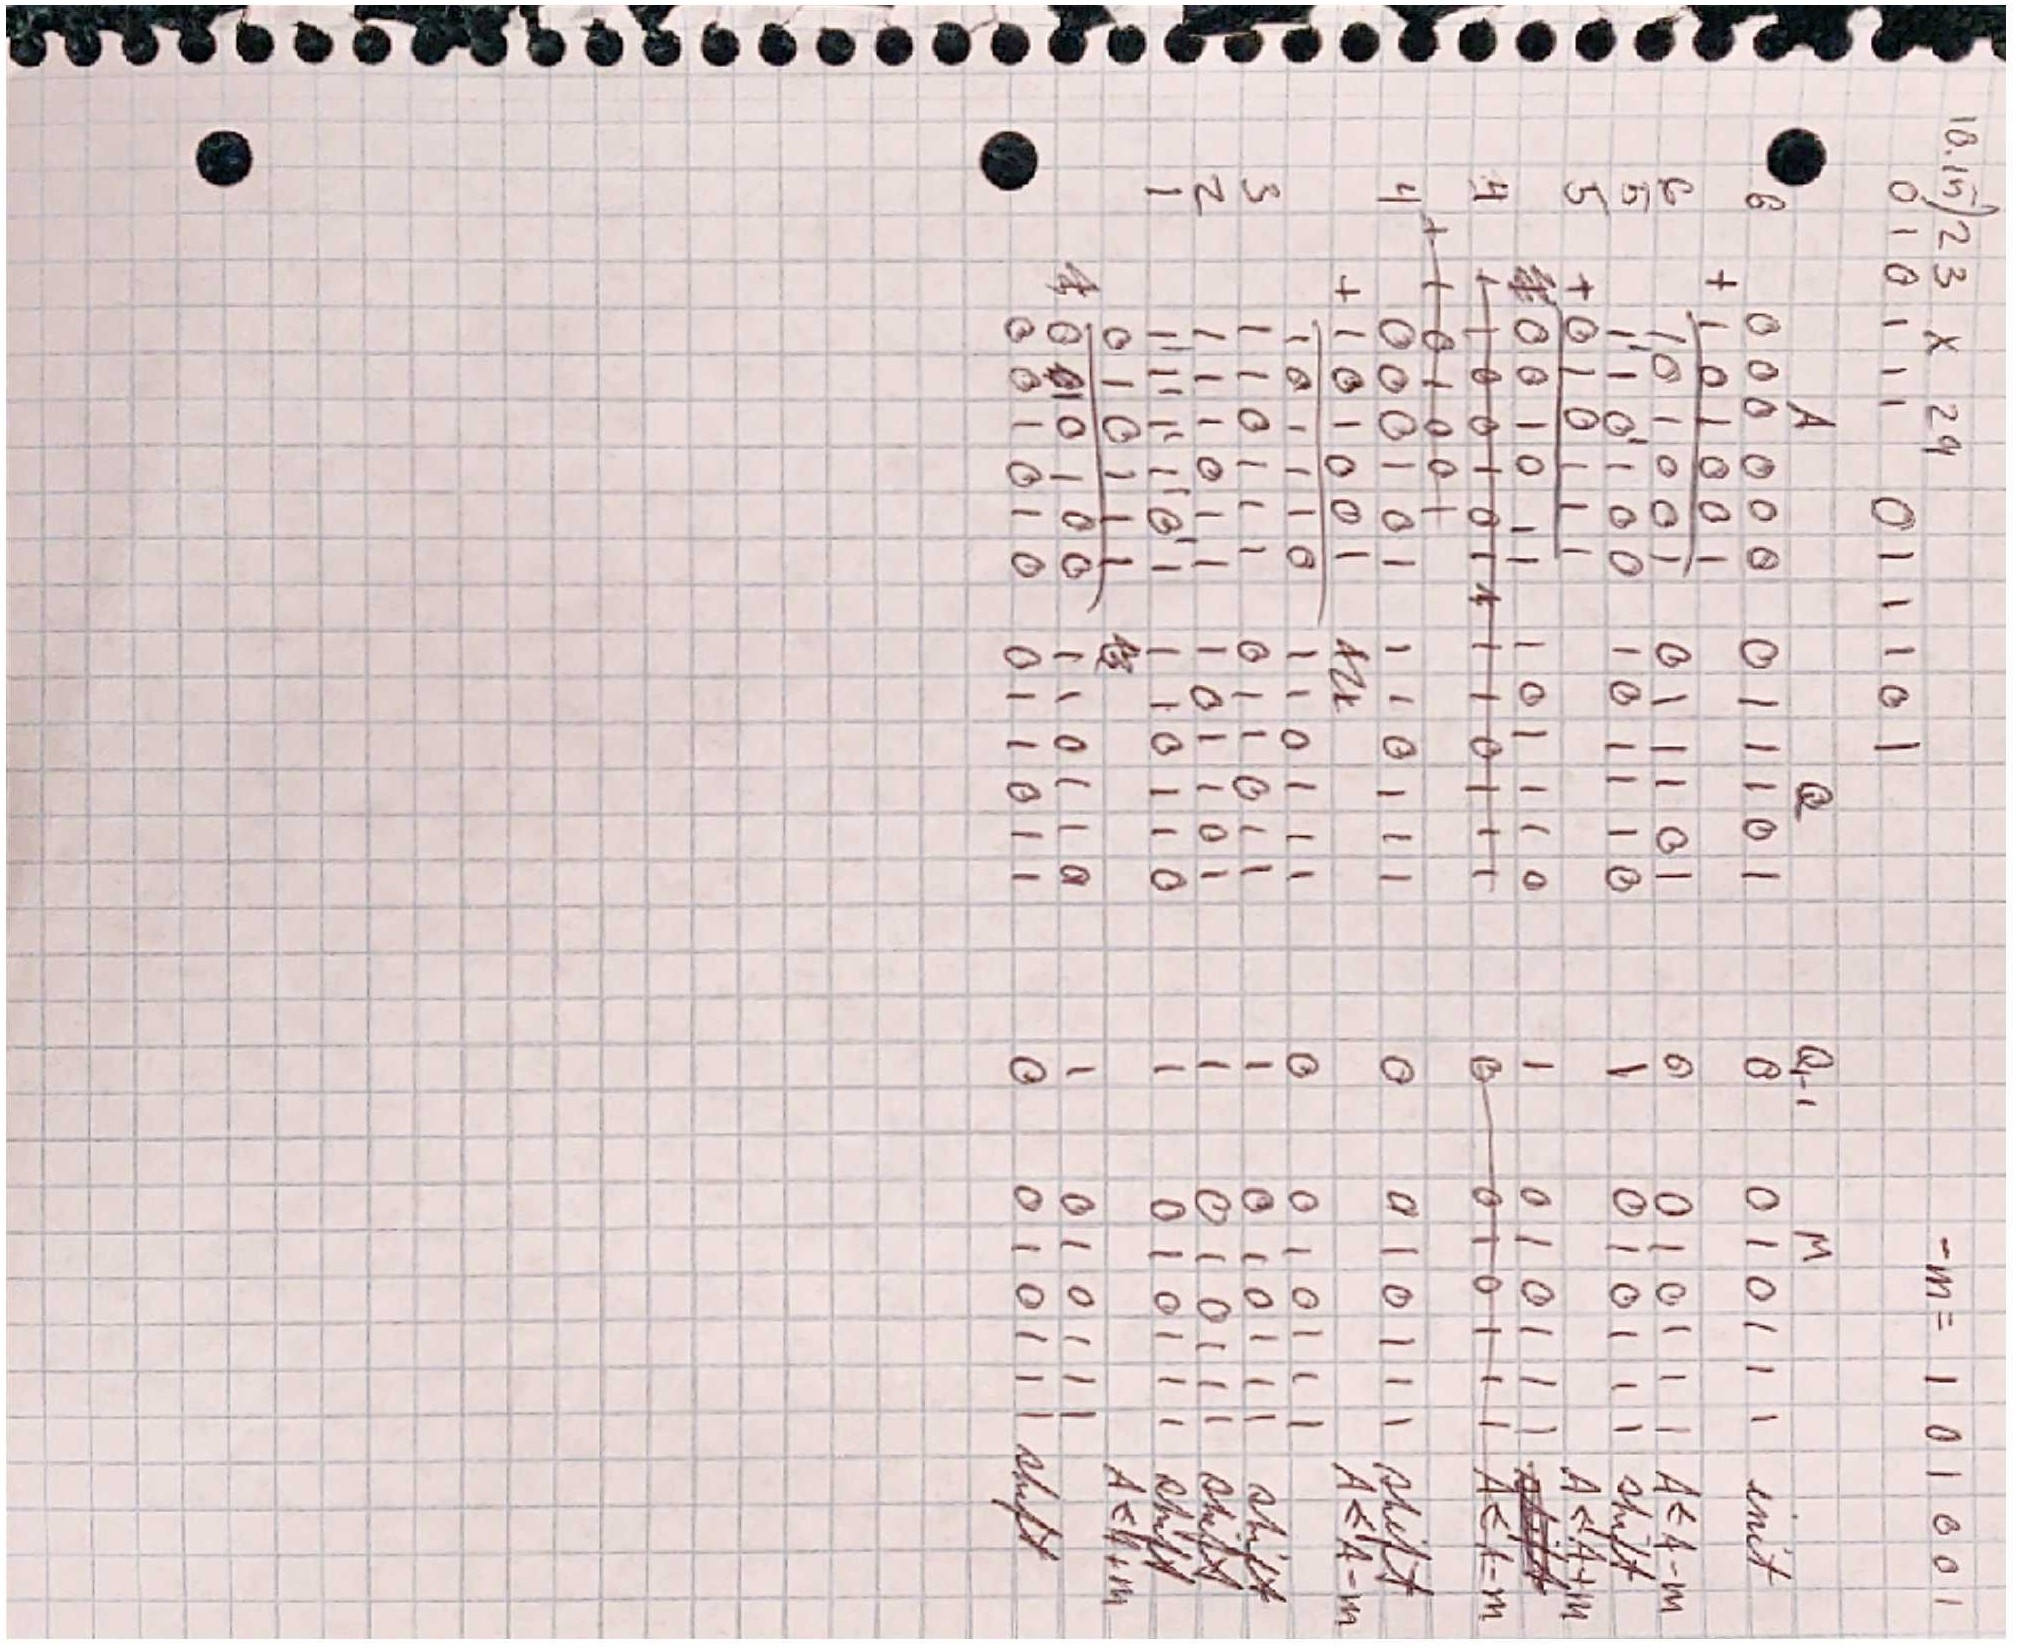
\includegraphics[scale=.25, angle=90]{homework1_10-15work}
\end{document}